\section{Implémentation des algorithmes}\label{sec:conception_implementation}

    Avant de pouvoir implémenter les nouveaux algorithmes, il a fallu récupérer un algorithme de calcul de \textit{core} car Graal n'en comprend pas encore (\ref{subsec:calcul_core}), et ensuite les nouveaux algorithmes ont pu être implémentés (\ref{subsec:implementation_chainage_avant}).
    
    \subsection{Le calcul du \textit{core}}\label{subsec:calcul_core}
     
     Graal ne comprenant pas d'algorithme pour calculer le \textit{core}, il a fallu en trouver une implémentation ailleurs. Il s'avère que l'un des participants à ce projet TER avait réalisé un stage dont l'un des buts était de développer de tels algorithmes pour Graal \cite{CORECHASE}. On va donc rapidement analyser son code source (\ref{subsubsec:analyse_existant_core}) avant de voir comment l'intégrer au projet (\ref{subsubsec:integration_core}).
    
    \subsubsection{Analyse de l'existant pour le calcul du \textit{core}}\label{subsubsec:analyse_existant_core}
    
     \par Durant ce stage, les classes de la figure \ref{fig:dclasse_existant_core} ont été réalisées.
     
        \begin{figure}[H]
        \centering
        \vspace{-10pt}
        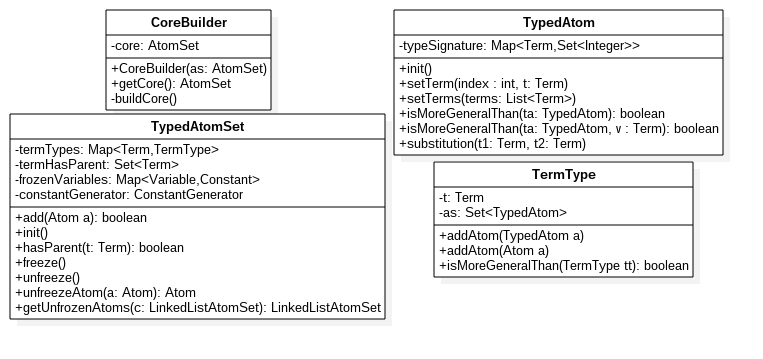
\includegraphics[width=\textwidth]{pictures/diag_classe_existant_core.png}
        \vspace{-35pt}
        \caption{Diagramme de classe de l'existant pour le \textit{core}}
        \vspace{-5pt}
        \label{fig:dclasse_existant_core}
        \end{figure}
     \par On va ne pas entrer dans les détails pour les classes \textbf{TypedAtomSet}, \textbf{TypedAtom} et \textbf{TermType}. Il faut juste savoir qu'elles sont utilisées par l'algorithme de calcul du \textit{core} et qu'il faudra donc les récupérer.
     \par La classe \textbf{CoreBuilder} est celle permettant de calculer le \textit{core} d'un ensemble d'atomes, qui sera passé en paramètre au constructeur. Une des caractéristiques de cette classe est que l'ensemble d'atomes passé en paramètre du constructeur est modifié, mais on ne veut pas forcément que ce soit le cas. Aussi, on pourrait vouloir un algorithme de calcul du \textit{core} totalement naïf pour les petits ensembles d'atomes : cette classe fait en effet beaucoup de pré-calculs et peut s'avérer plus lente sur de tels ensembles. On constatera également l'absence d'interface qui serait commune à tous les algorithmes de \textit{core}.
     \par Dans la section qui suit, les modifications apportées vont être détaillées.
     
    \subsubsection{Intégration du calcul du \textit{core} au projet}\label{subsubsec:integration_core}
    
    Tout d'abord, on va créer une interface commune à tous les algorithmes de \textit{core}. Cette interface devra prévoir les possibilités suivantes :
    \begin{itemize}
        \item on peut avoir le choix entre calculer le \textit{core} directement dans l'ensemble d'atomes passé en paramètre (méthode \textit{getCore}) ou dans un nouvel ensemble (méthode \textit{computeCore}) ;
        \item on peut choisir de fixer des variables, qui ne seront donc pas supprimées par le calcul du \textit{core} (gel des variables).
    \end{itemize}
    Cette interface sera implémentée par une classe \textbf{AbstractCore} qui contient des méthodes par défaut pour les différents algorithmes de \textit{core}. Cette classe est spécialisée par deux autres. La première est \textbf{ImprovedCore} calculant la version améliorée de l'algorithme de \textit{core} - il sagit donc de la classe \textbf{CoreBuilder} présentée précédemment, modifiée pour implémenter la nouvelle interface. La seconde est \textbf{NaiveCore}, calculant un algorithme de \textit{core} naïf ne faisant aucun pré-calcul.
    \par Le diagramme des nouvelles classes est disponible figure \ref{fig:dclasse_new_core}.
        \begin{figure}[H]
        \centering
        \vspace{-10pt}
        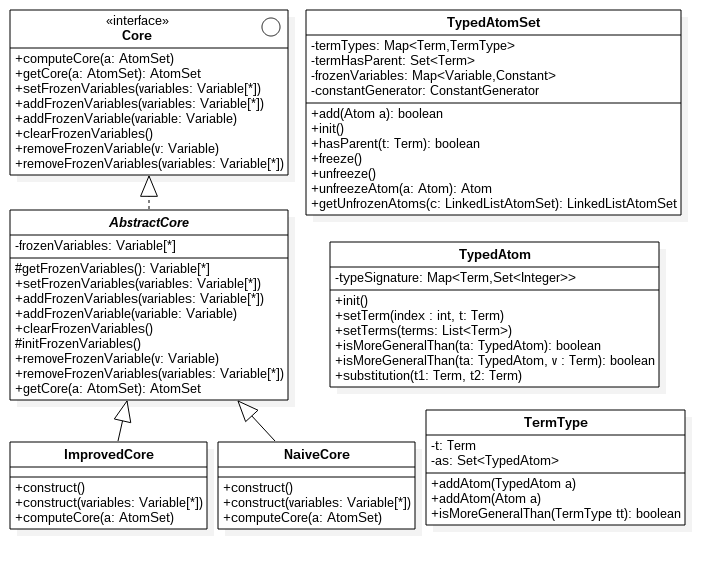
\includegraphics[width=\textwidth]{pictures/diag_classe_new_core.png}
        \vspace{-35pt}
        \caption{Diagramme de classe de l'intégration du \textit{core} au projet}
        \vspace{-5pt}
        \label{fig:dclasse_new_core}
        \end{figure}
     
    \subsection{Implémentation des algorithmes de chaînage avant}\label{subsec:implementation_chainage_avant}
    
    Avant de commencer à concevoir des classes en vue d'implémenter les algorithmes présentés précédemment, il faut procéder à une analyse de l'existant (\ref{subsubsec:analyse_existant_graal}). Puis la conception des nouvelles classes sera détaillé (\ref{subsec:implementation_dans_graal}).
    
     \subsubsection{Analyse de l'existant dans Graal}\label{subsubsec:analyse_existant_graal}
        % Il y a deux choses à analyser : d'abord, les algorithmes de chaînage avant existant déjà dans Graal (\ref{subsubsec:analyse_existant_graal}), puis les algorithmes de calcul du \textit{core} créés pour Graal (\ref{subsubsec:analyse_existant_core}).
    
       
        
        Comme présenté dans l'introduction, Graal est une bibliothèque en Java créée par l'équipe GraphiK pour pouvoir réaliser des calculs sur des bases de connaissance. Elle a été créée principalement dans le but d'implémenter des algorithmes efficaces de chaînage arrière. Les algorithmes de chaînage avant ne sont apparus que dans un second temps : cette bibliothèque n'a donc pas été conçue dès le départ pour ce type d'algorithme.
        \par Les différentes classes pour les chaînages avant se trouvent dans trois paquets différents : graal.api.forward\_chaining, graal.forward\_chaining et graal.grd.forward\_chaining. Le premier contient notamment toutes les interfaces, le second contient des implémentations des chaînage avant et enfin le dernier contient une forme spécifique de chaînage utilisant des graphes de dépendance des règles (\textit{graph rule dependency} ou \textit{grd}) pour déterminer l'ordre d'application des règles.
        \par On va détailler les paquets dans les paragraphes qui suivent. Un diagramme de classes complet de tous les paquets est disponible en annexe \ref{sec:dia_classe_existant}.
        
        \paragraph{Paquet graal.api.forward\_chaining} 
        
        \begin{figure}[H]
        \centering
        \vspace{-20pt}
        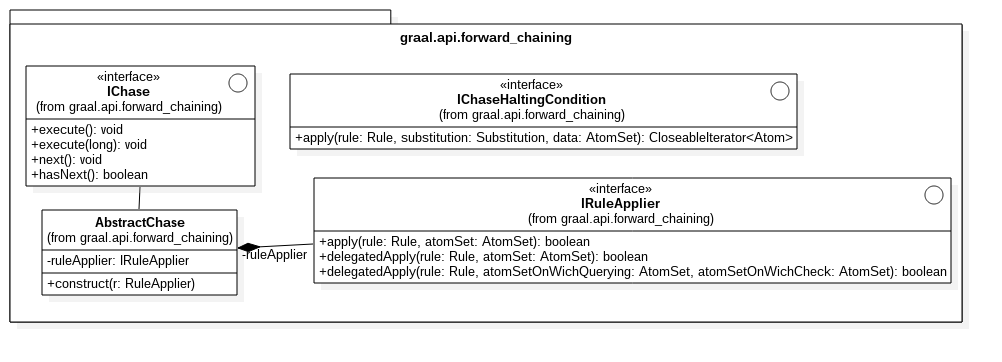
\includegraphics[width=\textwidth]{pictures/diag_class_api_forward_chaining.png}
        \vspace{-35pt}
        \caption{Diagramme de classes du paquet graal.api.forward\_chaining}
        \label{fig:dclasse_api_forward_chaining}
        \end{figure}
        Ce paquet est composé de 3 interfaces et une classe abstraite (figure \ref{fig:dclasse_api_forward_chaining}).
        \par L'interface \textbf{IChase} est l'interface qui doit être implémentée par tous les algorithmes de \textit{chase} de Graal. Elle est implémentée par la classe \textbf{AbstractChase}, qui est la classe mère de tous les algorithmes de chaînage avant implémentés dans Graal.
        \par L'interface \textbf{IRuleApplier} est une interface qui doit être implémentée par toutes les classes servant à appliquer des règles. Cependant, certaines classes appliquant les règles ne les applique pas totalement d'elles-même, elles font appel à une des classes implémentant l'interface \textbf{IChaseHaltingCondition}. Le nom de cette dernière semble assez mal choisi car il ne s'agit pas d'une condition d'arrêt des algorithmes de chaînage avant. Les classes implémentant cette interface réalisent des applications de déclencheurs qui leurs sont fournis par les classes d'application des règles, en testant un critère d'applicabilité. Donc non seulement le nom semble mal choisi, mais cette interface est implémentée par des classes faisant deux opérations différentes : test du critère d'applicabilité et application d'un déclencheur.
        
        \paragraph{Paquet graal.forward\_chaining}
        \begin{figure}[!h]
        \centering
        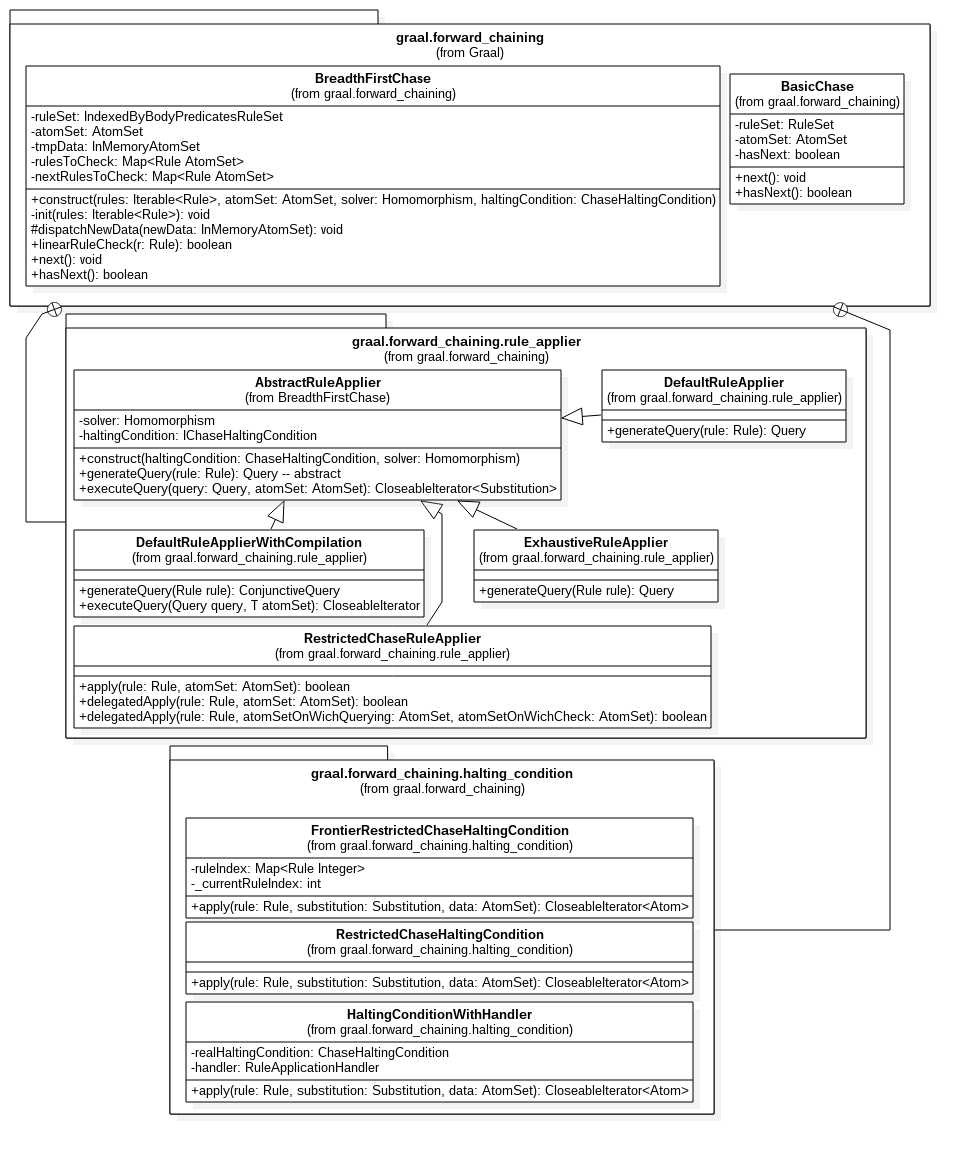
\includegraphics[width=\textwidth]{pictures/forward_chaining_class_diagram.png}
        \vspace{-30pt}
        \caption{Diagramme de classes du paquet graal.forward\_chaining}
        \label{fig:dclasse_forward_chaining}
        \end{figure}
        
         Ce paquet est composé de deux classes et deux sous-paquets (figure \ref{fig:dclasse_forward_chaining}). On va donc commencer par décrire les deux classes puis on va présenter les deux sous-paquets.
         \par La classe \textbf{BasicChase} est le premier algorithme de chaînage avant implémenté dans Graal. Il ne semble ni être un chaînage avant en profondeur, ni en largeur. Il s'agit probablement d'une implémentation ratée d'un chaînage avant en largeur. Cette classe n'est plus utilisée ailleurs dans la bibliothèque.
         \par La classe \textbf{BreadthFirstChase} quant à elle sert de base aux algorithmes de chaînage en avant en largeur implémentés dans Graal. Malheureusement, elle ne semble pas très optimale quant à sa manière de rechercher les nouveaux déclencheurs : elle recherche tous les homomorphismes sur la base de faits entière à chaque étape, ce qui fait qu'elle retrouve tous les homomorphismes déjà appliqués précédemment. Une exception à noter est une optimisation pour les règles linéaires (c'est-à-dire des règles ne contenant qu'un seul atome dans leur corps) : les homomorphismes ne sont cherchés que parmi les nouveaux faits de l'étape précédente. Cette classe est utilisée en combinaison avec les classes contenues dans les deux sous-paquets décrits ci-après pour obtenir le type de chaînage avant souhaité.
         
         \paragraph{Paquet graal.forward\_chaining.rule\_applier} Ce sous-paquet contient les applicateurs de règles. Il y a tout d'abord une classe abstraite \textbf{AbstractRuleApplier} qui sert de base à toutes les autres classes du paquet. Puis il y a quatres autres classes.
         \par La première est \textbf{ExhaustiveRuleApplier} qui applique tous les déclencheurs comme l'indique son nom. 
         \par La classe \textbf{DefautlRuleApplier} quant à elle modifie les déclencheurs : en effet, une fois les déclencheurs $(R,h)$ trouvés, elle réduit $h$ aux variables contenues dans la frontière de la règle $R$. Cela peut donc réduire le nombre de déclencheurs à tester et appliquer et également le nombre de redondances. 
         \par La classe \textbf{DefaultRuleApplierWithCompilation} fait la même chose mais fait une compilation des requêtes faites sur la base de faits pour trouver les homomorphismes. On ne va pas entrer dans les détails ici, mais il s'agit juste d'une manière d'optimiser les temps de calcul. 
         \par Enfin, le \textbf{RestrictedChaseRuleApplier} est un applicateur de règles conçu spécialement pour le \textit{restricted chase}. La requête servant à trouver les homomorphismes envoyant le corps de la règle dans la base de faits est accompagnée d'une partie négative contenant les atomes de la tête de la règle. Cela sert à n'obtenir que les déclencheurs respectant le critère d'applicabilité du \textit{restricted chase}. De ce fait, cette dernière classe ne fait pas appel aux classes du sous-paquet que l'on va présenter maintenant et qui s'occupe notamment de vérifier le critère d'applicabilité.
         
         \paragraph{Paquet graal.forward\_chaining.halting\_condition} Ce sous-paquet contient les classes implémentant l'interface \textbf{IChaseHaltingCondition} présentée précédemment. 
         \par La classe \textbf{FrontierRestrictedChaseHaltingCondition}, contrairement à ce que son nom pourrait laisser entendre, ne sert pas de base à un algorithme de \textit{restricted chase}, mais à un alogrithme de \textit{semi-obblivious chase}. \par C'est la classe \textbf{RestrictedChaseHaltingCondition} qui sert à construire un \textit{restricted chase}, dans les cas où l'on n'utilise pas le \textit{RestrictedChaseRuleApplier}.
         \par Enfin, le manque de documentation de la bibliothèque ne nous a pas permis de comprendre précisément l'utilité de la classe \textit{HaltingConditionWithHandler}.
         \par Cela n'étant pas forcément clair, avant de passer à la présentation du dernier paquet, il convient de détailler un peu plus comment se déroule l'application d'une règle lors d'une saturation, en revenant plus en détail sur la méthode \textit{next()} contenue dans la classe \textbf{BreadthFirstChase}.
         
         
         \paragraph{Méthode \textit{next()}}
        \begin{figure}[H]
        \centering
        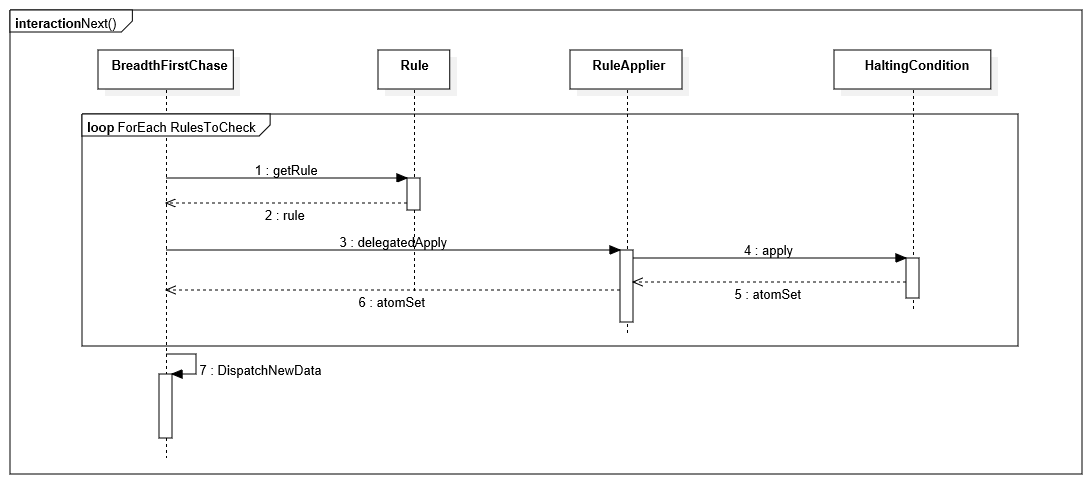
\includegraphics[width=\textwidth]{pictures/DiagrammeSequence.png}
        \caption{Diagramme de séquence next()}
        \label{fig:dsequence}
        \end{figure}
        
        La méthode \textit{next()} fait une étape de largeur de l'algorithme de chaînage avant en largeur (figure \ref{fig:dsequence}). Cette méthode utilise deux \textit{hashmaps} du type \textit{Map<Rule, AtomSet>} pour stocker les règles qui devront être appliquées à l'étape suivante et les atomes qui seront utilisés pour le calcul des homomorphismes, ces deux hashmaps s'appellent \textit{rulesToCheck} et \textit{nextRulesToCheck}. Avant le premier appel à la méthode on initialise \textit{nextRulesToCheck} avec toutes les règles de la base de règles de la façon suivante : $nextRulesToCheck({R}) = <\mbox{règle},\mbox{base de faits}> $. À chaque appel de la méthode \textit{next()} on suit les étapes suivantes : 
        \\
        
        \begin{itemize}
        \item On copie $nextRulesToCheck$ dans $rulesToCheck$, et on réinitialise $nextRulesToCheck$.
        \item Pour chaque règle $R_i$ dans $rulesToCheck$ on appelle la méthode $delegatedApply$ dans \textit{RuleApplier} qui va calculer tous les homomorphismes du corps de la règle vers la base de faits de l'étape précédente, puis, pour chacun des déclencheurs ainsi obtenus, on appelle la méthode $apply$ dans \textit{HaltingCondition} et on applique le déclencheur s'il respecte le critère d'applicabilité.
        \item Les atomes générés par \textit{HaltingCondition} sont renvoyés au \textit{BreadthFirstChase} à travers \textit{RuleApplier}. Ces atomes sont stockés par \textit{BreadthFirstChase} dans \textit{nouvFaits} puis on continue avec la règle suivante.
        \item Quand on a traité toutes les règles on appelle $dispatchNewData$ qui va faire deux chose différentes en fonction du type de chaque règle de la base de règles :
        \begin{itemize}
            \item Si la règle est linéaire (le corps ne contient qu'un seul atome), on prend les atomes dans les nouveaux faits qui ont le même prédicat et on les ajoute dans l'ensemble des atomes à partir duquel on calculera les nouveaux déclencheurs pour cette règle à l'étape suivante, dans \textit{nextRuleToCheck} ;
            \item Sinon, si le corps de la règle contient un atome dont le prédicat est aussi le prédicat d'un atome dans les nouveaux faits, alors on ajoute cette règle dans \textit{nextRuleToCheck} avec comme ensemble d'atomes sur lequel calculer les nouveaux déclencheurs la base de faits entière (les déclencheurs obtenus ne seront pas tous forcément nouveaux).
        \end{itemize}
        \end{itemize}
         
        
        \paragraph{Paquet graal.grd.forward\_chaining} 
        \begin{figure}[H]
        \centering
        \vspace{-15pt}
        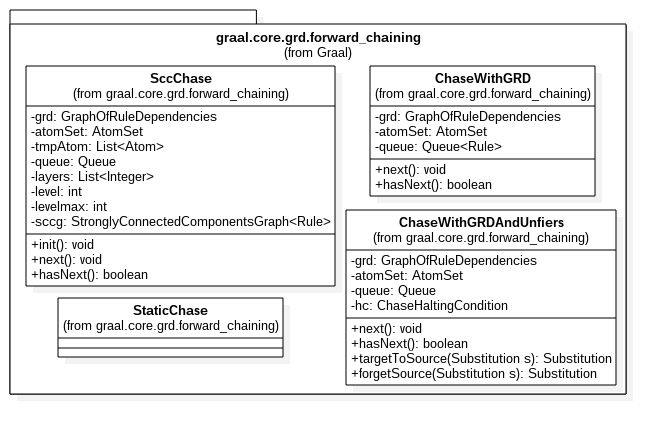
\includegraphics[width=0.8\textwidth]{pictures/diag_class_grd_forard_chaining.png}
        \vspace{-30pt}
        \caption{Diagramme de classes du paquet graal.grd.forward\_chaining}
        \label{fig:dclasse_grd_forward_chaining}
        \end{figure}
        Ce paquet contient des algorithmes de chaînage utilisant un graphe de dépendances des règles (figure \ref{fig:dclasse_grd_forward_chaining}). Ces algorithmes sont différents des chaînages avant en largeur auxquels nous nous intéressons dans le cadre de ce projet. On notera cependant une erreur dans le nom d'une classe (\textbf{ChaseWithGRDAndUnfiers} au lieu de \textbf{ChaseWithGRDAndUnifiers}) et une classe dont on se pose la question de l'utilité (\textbf{StaticChase}) puisqu'elle ne contient que des méthodes de classe permettant d'obtenir une instance de certains algorithmes de chaînage avant, sans que cela soit forcément plus intéressant que de créer une instance soi-même.
        
        \paragraph{Faut-il partir sur un nouveau paquet ?} Après avoir analysé l'existant dans Graal, on constate que les chaînages en avant implémentés présentent beaucoup de défauts. Un défaut qui n'a pas été évoqué jusqu'à maintenant, c'est le manque de flexibilité de cette implémentation : il n'est par exemple pas possible de pouvoir changer facilement l'extension globale et l'extension locale ce qui est pourtant nécessaire à l'implémentation de certains des algorithmes présentés dans ce rapport. À cela, il faut ajouter que certaines classes méritent un renommage.
        \par C'est en raison de tous les défauts évoqués dans cette section que la décision a été prise d'implémenter les algorithmes de chaînage avant présentés dans un nouveau paquet \textit{graal.new\_forward\_chaining} comme cela sera présenté dans la section qui suit.
        
        % Dans cette partie nous analysons ce qui était déjà présent sur GRAAL pour les \textit{chases}.
        
        % Le package graal-forward-chaining est compris par 3 packages :
        % \begin{itemize}
        %     \item \textit{Chase} : Il contient les implémentations des différentes \textit{chases} ( BreadthFirst, GRD, etc )
        %     \item \textit{HaltingCondition} : Une halting condition sert à tester si un trigger (R,h) est "actif" et s'il l'est la règle est appliquée par rapport à h.
        %     \item \textit{RuleApplier} : Un rule applier sert à calculer tous les homomorphismes du Body d'une règle dans F et ensuite il utilise les homomorphismes trouvés pour appliquer la règle en utilisant une \textit{HaltingCondition}.
        % \end{itemize}
        
       % \paragraph{Package Chase}\ \\
        % Le package \textit{Chase} est compris d'une interface \textit{IChase} étant implementé par tous les \textit{chases} dans GRAAL. D'une classe abstraite AbstractChase qui implemente des versions génériques pour les méthodes de \textit{chases}. Enfin on a les différentes classes implementant different type de \textit{chases}.\\
        % Le \textit{BasicChase} est une implémentation basique du \textit{chases} en largeur sans aucune optimisation. \\
        % Le \textit{BreadthFirstChase} est une implémentation optimisée du \textit{chase} en largeur. Une première optimisation est l'utilisation de \textit{nouvFaits} à la fin de chaque étape pour déterminer quelles règles seront déclenchées à l'étape prochaine. On détermine aussi parmi ces règles lesquelles sont linéaires (avec un seul atome dans le body) pour stocker les atomes à utiliser pour le calcul des homomorphismes de façon à ce que ce dernier prenne en entrée une petite collection d'atomes plutôt que la base la base de faits entière. \\
        % Le \textit{ChaseWithGRD} est un \textit{chase} qui utilise le graphe de dépendance des règles.\\
        % Le \textit{SccChase} est un \textit{Chase} qui sature chaque composante fortement connexe du graphe de dépendance des règles individuellement. on l'utilise par la classe statique \textit{StaticChase}.\\
        % Enfin le \textit{ChaseWithGRDAndUnfiers} est un \textit{chase} utilisant le graphe de dépendance des règles et des unificateurs.
        
        %\begin{itemize}
            %\item IChase : Interface qui doit être implémenté par tous les chases dans GRAAL.
            %\item AbstractChase : Classe abstraite qui implémente des versions génériques pour les méthodes des chases.
            %\item BasicChase : Implémentation basique du chase en largeur sans aucune optimisation.
            %\item BreadthFirstChase : Implémentation optimisée du chase en largeur. Une première optimisation est l'utilisation de nouvFaits à la fin de chaque étape pour déterminer quelles règles seront déclenchées à l'étape prochaine. On détermine aussi parmi ces règles lesquelles sont linéaires (avec un seul atome dans le body) pour stocker les atomes à utiliser pour le calcul des homomorphismes de façon à ce que ce dernier prenne en entrée une petite collection d'atomes plutôt que la base la base de faits entière.
            %\item ChaseWithGRD : Chase qui utilise le graphe de dépendance des règles.
            %\item SccChase : Chase qui sature chaque composante fortement connexe du graphe de dépendance des règles individuellement.
            %\item StaticChase : Classe statique qui permet d'utiliser le SccChase.
            %\item ChaseWithGRDAndUnfiers : Chase utilisant le graphe de dépendance des règles et des unificateurs.
        %\end{itemize}
        
        % \paragraph{Package Halting Condition}\ \\
        % Le package \textit{Halting Condition} permet normalement de définir les différentes conditions d'arrêt pour la saturation des \textit{chases}. Mais ici un Halting condition teste plutôt si un déclencheur est actif avant de l'appliqué le cas échéant.\\ 
        % Il est composé de l'interface \textit{IChaseHaltingCondition} qui est implémenté par toutes les halting conditions. On ainsi deux classes:\\
        % La \textit{FrontierRestrictedChaseHaltingCondition} est utilisée par le \textit{semi-oblivious chase}. \\
        % La \textit{RestrictedChaseHaltingCondition} est utilisée par le \textit{restricted chase}.
        %\begin{itemize}
            %\item IChaseHaltingCondition : Interface à implémenter pour toutes les halting conditions. 
            %\item FrontierRestrictedChaseHaltingCondition : HaltingCondition utilisée par le semi-oblivious chase.
            %\item RestrictedChaseHaltingCondition : HaltingCondition utilisée par le restricted chase.
        %\end{itemize}

        % \paragraph{Package RuleApplier}\ \\
        % Le package \textit{RuleApplier} est le package qui définit comment se s'applique les règles lors d'un \textit{chase}. Il est composé de l'interface \textit{IRuleApplier} qui est implementée par tous les \textit{rules appliers}. Nous avons ici 4 classes de \textit{rule applier}:\\
        % Le \textit{DefaultRuleApplier} calcule tous les homomorphismes puis ne garde que la frontière de chacun.\\
        % L'\textit{ExhaustiveRuleApplier} calcule tous les homomorphismes et les garde sans aucune modification.\\
        % Le \textit{RestrictedChaseRuleApplier} est spécifiquement optimisé pour le \textit{restricted chase}.\\
        % Le \textit{DefaultRuleApplierWithCompilation} est un \textit{Rule Applier} qui utilise des règles avec compilation.
        
        %\begin{itemize}
            %\item IRuleApplier : Interface à implémenter pour tous les rules appliers. 
            %\item DefaultRuleApplier : Il calcule tous les homomorphismes puis ne garde que la frontière de chacun.  
            %\item ExhaustiveRuleApplier : Il calcule tous les homomorphismes et les garde sans aucune modification.
            %\item RestrictedChaseRuleApplier : Rule Applier spécifiquement optimisé pour le restricted chase. 
            %\item DefaultRuleApplierWithCompilation : Rule Applier qui utilise des règles avec compilation.
        %\end{itemize}
        
        
        
        % \paragraph{Critique}
        % Face à cette organisation et dans l'idée de proposer notre propre itération d'une implémentation des \textit{chases}  nous avons donc était amené à nous demandé qu'elles étaient les choses pouvant être améliorées.\\
        % Tout d'abord le nom du package \textit{HaltingCondition} n'est pas le plus clair, une \textit{halting condition} devrait normalement être une condition d'arrêt pour la saturation d'un \textit{chase}, mais ici, elles testent si un trigger est actif et ensuite l'appliquent.\\
        % Ensuite nous avons remarqué que l'implémentation génériques des \textit{chases} n'utilisé pas les notions d'extensions locale et d'extensions globale, GRAAL fait toujours l'union ce qui pourrait être amélioré.\\
        % Nous avons aussi remarqué qu'il existe des classes qui ne sont pas utiles ou pas encore finies. \textit{StaticChase} ou \textit{HaltingConditionWithHandler} en sont des exemples.\\
        % Enfin nous nous sommes rendus compte que dans l'implémentation actuelle de Graal, les homomorphismes sont recalculés intégralement à chaque étape du \textit{chase}, ce qui ralentit considérablement le calcul de la base de faits saturée.
        %\begin{itemize}
            %\item Nous ne trouvons pas que le package HaltingCondition est bien nommé, une halting condition devrait normalement être une condition d'arrêt pour la saturation d'un chase, mais ici, elles testent si un trigger est actif et ensuite l'appliquent.
            %\item Pour avoir des implémentions vraiment génériques des chases il faudrait rajouter les notions d'extension locale et d'extension globale, Graal fait toujours l'union.
            %\item Il existe des classes qui ne sont pas utiles ou pas encore finies. StaticChase ou HaltingConditionWithHandler en sont des exemples. 
            %\item Dans l'implémentation actuelle de Graal, les homomorphismes sont recalculés intégralement à chaque étape du chase, ce qui ralentit considérablement le calcul de la base de faits saturée.
        %\end{itemize}
        
        %\subsubsection{Conception}
     %\subsection{Conception et implémentation des simplificateurs de bases de règles}
     
     
     
    \subsubsection{Implémentation des nouveaux algorithmes de chaînage avant}\label{subsec:implementation_dans_graal}
       
       La structure de la nouvelle implémentation (diagramme de classe annexe \ref{sec:dia_classe_nouveau}) se base sur les algorithmes qui ont présentés dans la section \ref{sec:types_de_chases}. Ainsi, il y a un paquet comprenant l'algorithme générique de chaînage en avant (\textit{new\_forward\_chaining.breadth\_first}), un paquet pour les algorithmes d'extension (\textit{new\_forward\_chaining.extender}) et un autre pour les critères d'applicabilité (\textit{new\_forward\_chaining.trigger\_checker}).
       \par Pour donner plus de flexibilité à la structure, un paquet \textit{new\_forward\_chaining.rule\_applier} a été ajouté : il comprend des classes dont le rôle est de calculer les déclencheurs pour une règle donnée, puis, à l'aide des classes appropriées, de tester le critère d'applicabilité et réaliser l'extension locale.
       \par Enfin, il est possible d'ajouter des conditions d'arrêt aux chaînages avant (paquet \textit{new\_forward\_chaining. halting\_condition}) et de leur faire faire des pré-calculs avant de lancer la saturation (paquet \textit{new\_forward\_chaining. pretreatment}).
       \par Mais avant cela, on va détailler le contenu du paquet contenant une définition de ce qu'est un \textit{chase}.
       
       \paragraph{Paquet new\_forward\_chaining} Il comprend une interface \textbf{Chase} définissant l'interface que doit implémenter tout algorithme de chaînage avant et une classe abstraite \textbf{AbstractChase} contenant quelques méthodes par défaut (figure \ref{fig:new_forward_chaining}). Cela va servir de base aux algorithmes de chaînage avant en largeur.
       
       \begin{figure}[h]
        \centering
        \vspace{-10pt}
        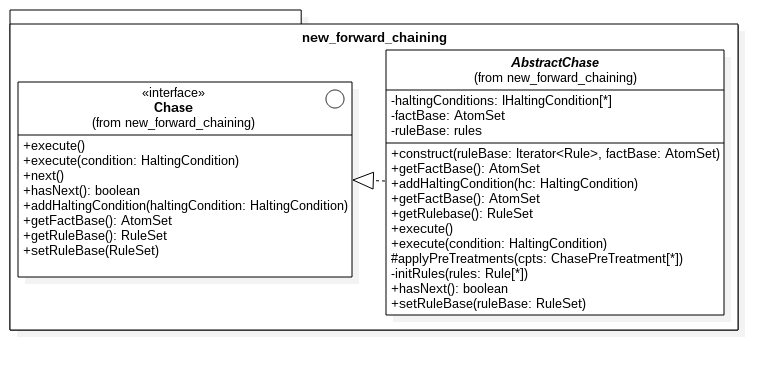
\includegraphics[width=0.8\textwidth]{pictures/new_forward_chaining.png}
        \vspace{-20pt}
        \caption{Diagramme de classes du paquet graal.grd.new\_forward\_chaining}
        \label{fig:new_forward_chaining}
        \vspace{-15pt}
        \end{figure}
       
       \paragraph{Paquet new\_forward\_chaining.breadth\_first} C'est ici que l'algorithme générique présenté en section \ref{sec:types_de_chases} est implémenté (figure \ref{fig:new_forward_chaining.breadth_first}). Il y a tout d'abord une interface \textbf{BreadthFirstChase}, spécialisant l'interface \textbf{Chase}, qui définit ce qu'est un algorithme de chaînage en largeur.
       \par On distingue deux types de chaînage avant en largeur : en parallèle (classe \textbf{ParallelBreadthFirstChase}) et pas en parallèle (classe \textbf{NotParallelBreadthFirstChase}) comme cela a été vu lorsque l'algorithme de \textit{restricted chase} a été présenté. La différence entre les deux classes se fait au niveau de l'ensemble d'atomes auquel aura accès le critère d'applicabilité : soit la base de faits de l'étape en cours, soit celle-ci à laquelle on ajoute les atomes des nouveaux faits. Les éléments communs à ces deux classes sont regroupés dans la classe \textbf{AbstractBreadthFirstChase} qu'elles spécialisent. Ces classes font appel, pour chaque règle, à un applicateur de règles.
       
       \begin{figure}[h]
        \centering
        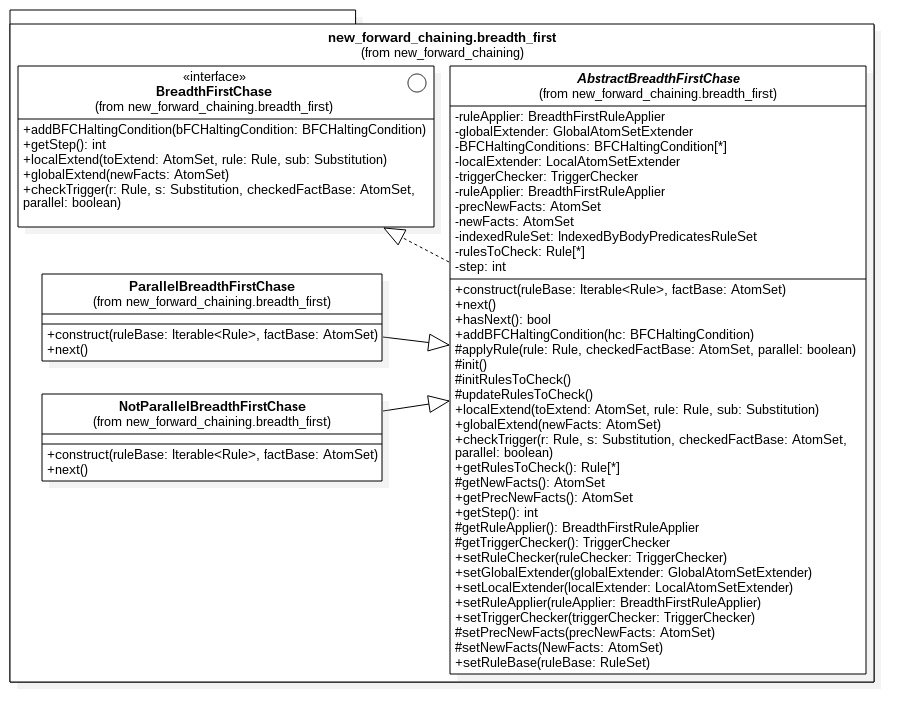
\includegraphics[width=\textwidth]{pictures/new_forward_chaining-breadth_first.png}
        \vspace{-35pt}
        \caption{Diagramme de classes du paquet graal.grd.new\_forward\_chaining.breadth\_first}
        \label{fig:new_forward_chaining.breadth_first}
        \vspace{-10pt}
        \end{figure}
        
       \paragraph{Paquet new\_forward\_chaining.rule\_applier} Il contient notamment la classe \textbf{DefaultBreadthFirstRuleApplier} qui est l'applicateur de règles par défaut pour le chaînage en avant en largeur (figure \ref{fig:new_forward_chaining.rule_applier}). Il intègre directement deux optimisations : il ne calcule que les déclencheurs qui sont nouveaux et il réduit directement l'homomorphisme qu'ils contiennent à leur frontière. Cela réduit donc le temps de calcul et permet de filtrer d'éliminer directement certaines redondances, avant même d'utiliser le critère d'applicabilité. Cette classe fait appel au critère d'applicabilité fournit par la classe qui l'utilise.
       
       \begin{figure}[h]
        \centering
        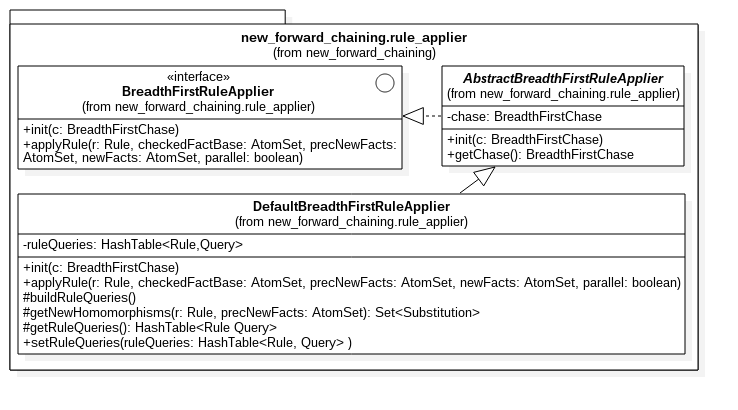
\includegraphics[width=0.85\textwidth]{pictures/new_forward_chaining-rule_applier.png}
        \vspace{-30pt}
        \caption{Diagramme de classes du paquet graal.grd.new\_forward\_chaining.rule\_applier}
        \label{fig:new_forward_chaining.rule_applier}
        \vspace{-10pt}
        \end{figure}
       
       \paragraph{Paquet new\_forward\_chaining.trigger\_checker} Les 3 critères d'applicabilité qui ont été présentés sont implémentés chacun dans leur propre classe : \textbf{ObliviousTriggerChecker}, \textbf{SemiObliviousTriggerChecker} et \textbf{RestrictedTriggerChecker} (figure \ref{fig:new_forward_chaining.trigger_checker}). Chacune de ces classes spécialisent la précédente car elles vérifient le critère de leur classe mère avant de vérifier le leur. En effet, par exemple, pour le \textit{restricted chase}, il est intéressant de d'abord vérifier le critère du \textit{semi-oblivious chase} car celui-ci est moins coûteux à calculer. Ainsi, si ce dernier n'est pas respecté, on évite le calcul de l'homomorphisme nécessaire au test d'applicabilité du \textit{restricted chase}, ce qui permet de l'optimiser. 
       \par Après avoir testé le critère d'applicabilité, il faut réaliser l'extension locale.
       
       \begin{figure}[h]
        \centering
        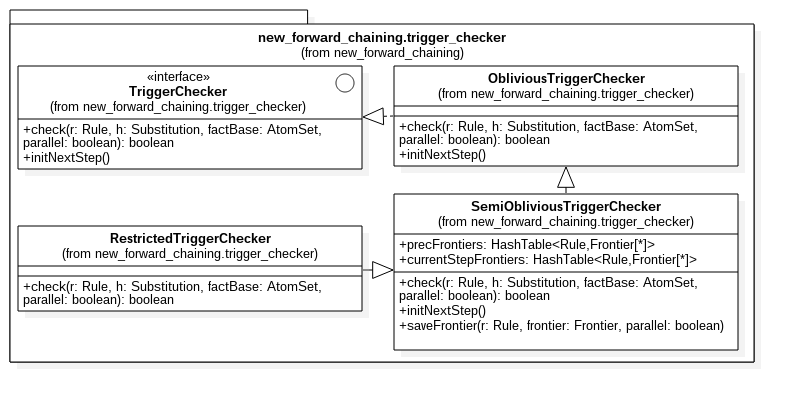
\includegraphics[width=0.85\textwidth]{pictures/new_forward_chaining-trigger_checker.png}
        \vspace{-30pt}
        \caption{Diagramme de classes du paquet graal.grd.new\_forward\_chaining.trigger\_checker}
        \label{fig:new_forward_chaining.trigger_checker}
        \end{figure}
       
       \paragraph{Paquet new\_forward\_chaining.extender}
       
       Comme il y a deux types d'algorithme d'extension, on distingue deux interfaces : \textbf{GlobalAtomSetExtender} et \textbf{LocalAtomSetExtender} (figure \ref{fig:new_forward_chaining.extender}). Puis, chaque algorithme d'extension a sa propre classe. La classe \textbf{DefaultAtomSetExtender} sert d'algorithme d'extension locale et globale pour l'\textit{oblivious chase} et tous les types d'algorithme utilisant les extensions globale et locale de l'\textit{oblivious chase}.
       \par La classe \textbf{CoreAtomSetExtender} contient l'algorithme d'extension globale pour le \textit{core chase}, en laissant le choix de l'algorithme de \textit{core} à utiliser, et la classe \textbf{LocalCoreChaseAtomSetExtender} est l'équivalent pour le \textit{local core chase}.
       \par Pour le \textit{vacuum chase}, la version est implémentée est la version A, mais seulement l'extension globale. En effet, comme expliqué dans la section \ref{sec:vacuum_chase}, l'extension locale spécifique au \textit{vacuum chase} n'est pas nécessaire lorsque les règles sont mono-pièces. On utilisera donc, comme on va le voir dans le paragraphe qui suit, un pré-traitement transformant les règles en règles mono-pièces.
       
       \begin{figure}[h]
        \centering
        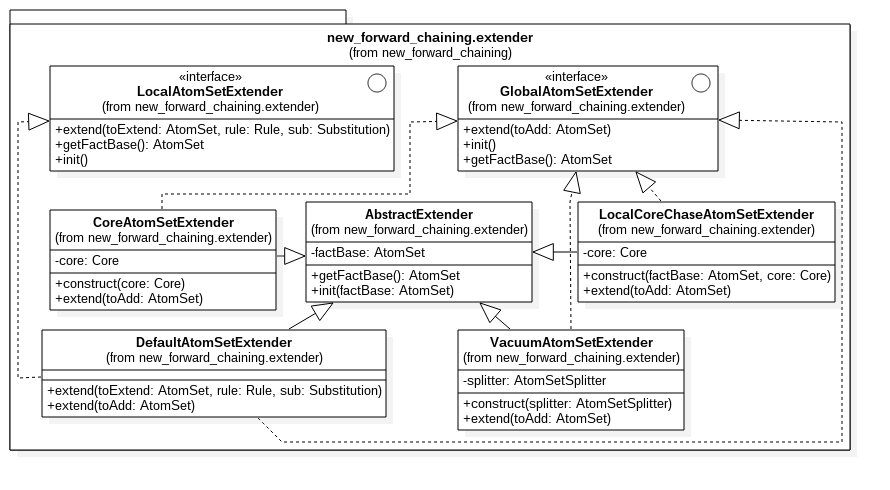
\includegraphics[width=\textwidth]{pictures/new_forward_chaining-extender.png}
        \vspace{-30pt}
        \caption{Diagramme de classes du paquet graal.grd.new\_forward\_chaining.extender}
        \label{fig:new_forward_chaining.extender}
        \end{figure}
       
       \paragraph{Paquet new\_forward\_chaining.pretreatment} Les pré-traitements sont des classes contenant un algorithme qui sera exécuté avant le début de la saturation. Deux pré-traitements ont été implémentés. Tout d'abord, un calcul du \textit{core} de la base de faits (classe \textbf{ComputeCore}), notamment utile avant le lancement d'un \textit{core chase} ou d'un \textit{local core chase}. Ensuite, un algorithme rendant les règles monopièces (classe \textbf{RuleSplit}), notamment à utiliser au début d'un \textit{vacuum chase}, mais aussi au début d'un \textit{restricted chase} car cela lui permet de supprimer plus de redondances (en effet, il peut arriver que seule une pièce de la tête puisse s'envoyer sur la base de faits mais pas la totalité - d'où le fait que rendre une règle monopièce puisse réduire le nombre de redondances).
       
       \paragraph{Paquet new\_forward\_chaining.halting\_condition} Le dernier paquet est celui des conditions d'arrêt. Deux conditions d'arrêt supplémentaires ont été implémentées : un arrêt au bout d'un temps limite (classe \textbf{TimeoutHaltingCondition}) et, dans le cas spécifique d'un chaînage avant en largeur, un arrêt au bout d'un nombre d'étapes limite (classe \textbf{LimitStepsHaltingCondition}).
       
       \paragraph{Paquet atom\_set\_splitter} Un paquet spécifique contenant des classes calculant les pièces d'un ensemble d'atomes a été ajouté. Il est notamment utile pour l'extension globale du \textit{vacuum chase} et le découpage des règles en règles mono-pièces. Il contient notamment la classe \textbf{DefaultAtomSetSplitter} qui réduit le problème de calculer les pièces d'un ensemble d'atomes à un problème de calcul de composantes connexes d'un graphe afin de pouvoir utiliser un algorithme en temps polynomial qui résout ce problème.
       
       \par~\par Ce projet a donc été l'occasion d'implémenter des algorithmes de chaînage avant n'existant pas dans Graal et de proposer une nouvelle structuration, plus flexible, permettant de réaliser facilement des ajouts et optimisations dans le futur. Ces implémentations ont permis de réaliser des comparaisons entre les différents types d'algorithme comme cela va maintenant être présenté.
       
       
%       \par~ \par~ \par~ \par~
%     \par Dans cette partie nous développerons le travail que nous avons fait sur l’implémentation des différents chases que nous proposons. 

% Il y a plusieurs façons pour exécuter un \textit{chase} (profondeur, largeur, parallèle), presque tout le travail était fait en utilisant les exécutions en largeur mais le paquet de \textit{chase} était fait pour être plus flexible et plus facile a intégrer les autres (profondeur et parallèle) plusieurs classes étaiement crées pour réaliser l'exécution \textit{chase} par largeur et une variante parallèle en largeur. Par rapport aux types de \textit{chases}, il faut tester l'applicabilité. Comme déjà expliquer le critère d'applicabilité diffère avec chaque type de \textit{chase} alors un paquet \textit{TriggerChecker} est fait. Et chaque type de \textit{chase} a une classe correspondante dans \textit{TriggerChecker}. Pour les algorithmes des \textit{chases} une des amélioration était l'utilisation de extension locale et l'extension globale, d'où vient la raison de créer le paquet \textit{Extender}.
% Et comme préciser précédemment, l'extension parfois diffère entre les types de chases et donc pour chaque extension différente utilisée une classe correspondante était crée. 
% Mais tout cela sera détaillé dans la section qui suit. 

% Après les test d'applicabilité le paquet \textit{ruleApplier} est utilisée. Dans un \textit{chase} choisi et après la vérification d'un trigger proposé on passe à l'application pour la création des nouveaux atomes, et possiblement leur ajout dans la base de fait. Avec l'utilisation des règles existentielle l'exécution des chases risque de ne pas s'arrêter. Pour éviter un tel problème des conditions d'arrêts ont été ajoutées. Plusieurs conditions d'arrêts par exemple le temps qui est fait dans la classe \textit{timeoutHaltingConditiong} et le nombre d'étapes dans \textit{LimitStepHaltingCondition}, il y a aussi le nombre limite d'atome. Alors dans le paquet \textit{HaltingCondition}, chaque type de condition était fait dans une classe. Enfin il y a le paquet \textit{core} qui a été créé pour l'application de l'algorithme du improvedCore qui est la version améliorée du core. De plus ce paquet contient le naiveCore qui est utilisé aussi pour l'élimination de redondances dans une règles. Mais on parlera plus précisément dans les sections qui suit  
    
%     %L'organisation des classes, les fonctions utilisées et de manière générale les problèmes que nous avons rencontré et au final comment cette nouvelle version est sensée fonctionner.
    
%     \paragraph{Package Chase}\ \\
%     Pour l'implémentation des \textit{chases} nous avons mis en place une interface Chase reprenant les fonctions \textit{execute()} et \textit{execute(HaltingCondition)} servant à exécuter l'algorithme \textit{chase} en ajoutant un condition d'arrêt.
%     Cette interface est héritée par la classe abstraite \textit{AbstractChase} qui implémente les versions générique des \textit{chases}. On a aussi l'interface \textit{BreadthFirstChase} (resp. \textit{DepthFirstChase}) qui représente l'interface qui doit être implémentée par les \textit{chases} en largeur (resp.profondeur).
%     Enfin on a la classe \textit{classicBreadthFirstChase} fonctionnant pour les exécutions en largeur et la classe \textit{ParralelBreadthFirstChase} fonctionnant pour les exécutions en parallèle. On a fait la différence entre les deux parce que la version en parallèle n’est pas affecté par l’ordre d’application de règles alors qu'une version en largeur est sensible à l’ordre d’application de règles.
%         %\begin{itemize}
%             %\item Chase : Interface qui doit être implémentée par tous les chases dans GRAAL.
%             %\item AbstractChase : Classe abstraite qui implémente des versions génériques pour les méthodes des chases.
%             %\item DepthFirstChase : Interface qui doit être implémentée par tous les chases en profondeur.
%             %\item BreadthFirstChase : Interface qui doit être implémentée par tous les chases en largeur.
%             %\item AbstractBreadthFirstChase : Classe abstraite qui implémente des versions génériques pour les méthodes des chases en largeur.
%             %\item ParallelBreadthFirstChase : Classe qui implémente les chases en parallèle.
%             %\item NotParallelBreadthFirstChase : Classe qui implémente les chases en largeur.
%         %\end{itemize}
        
%     \paragraph{Package Trigger Checker}\ \\
%     Pour le test d'applicabilité des règles nous avons mis en place une interface \textit{TriggerChecker} reprenant la fonction \textit{check} qui nous répond par vrai si une règle donnée est applicable pour un homomorphisme et la base de faits données et faux sinon. Et nous avons différentes classes pour les différents implémentations pour le test d'applicabilité. La classe qui vérifie l'applicabilité de l'\textit{Oblivious chase} par la méthode check et donc va retourner toujours vrai. Voir l'algorithme \ref{algo:est_applicable_oblivious}. La classe qui étend l'\textit{ObliviousTriggerChecker} en vérifiant l'applicabilité du \textit{SemiOblivious chase} par la méthode check. Voir l'algorithme \ref{algo:est_applicable_semi_oblivious}. Et finallement la classe qui étend le \textit{SemiObliviousTriggerChecker} en  vérifiant l'applicabilité du \textit{Restricted chase} par la méthode \textit{check}. Voir l'algorithme \ref{algo:est_applicable_restricted_largeur}.
%         \\
%         %\begin{itemize}
%             %\item TriggerChecker : Interface qui doit être implémenté par tous les TriggerChecker dans GRAAL.
%             %\item ObliviousTriggerChecker : Classe qui vérifie l'applicabilité de l'Oblivious chase par la méthode check. Voir l'algorithme \ref{algo:est_applicable_oblivious}. % retourne toujours vrai
%             %\item SemiObliviousTriggerChecker : Classe qui étend l'ObliviousTriggerChecker en  vérifiant l'applicabilité du SemiOblivious chase par la méthode check. Voir l'algorithme \ref{algo:est_applicable_semi_oblivious}.
%             %\item RestrictedTriggerChecker : Classe qui étend le SemiObliviousTriggerChecker en  vérifiant l'applicabilité du Restricted chase par la méthode check. Voir l'algorithme \ref{algo:est_applicable_restricted}.
%         %\end{itemize}
        
%     \paragraph{Package Halting Condition}\ \\
%     Pour éviter les cas où l'exécution d'un \textit{chase} ne termine pas, nous avons dû ajouter une condition d'arrêt. On a mis en place une interface \textit{HaltingCondition} (resp. \textit{BFCHaltingCondition}) reprenant la fonction \textit{isFinished} qui nous dit si l'exécution des \textit{chases} (resp. \textit{chases} en largeur) est terminée ou non. \textit{HaltingCondition} (resp. \textit{BFCHaltingCondition}) est héritée par la classe abstraite \textit{AbstractHaltingCondition} (resp. \textit{AbstractBFCHaltingCondition}) qui implémente les conditions d'arrêt pour les différents \textit{chases} (resp. \textit{chases} en largeur). On a deux conditions d'arrêt la première consiste à tester si l'exécution a dépassé un certain nombre d'étapes c'est pourquoi on a la classe \textit{LimitStepsHaltingCondition} et la seconde avec la classe \textit{TimeoutHaltingCondition} consiste à tester si l'exécution a dépassé un certain temps donné.
%         %\begin{itemize}
%             %\item HaltingCondition : Interface qui doit être implémentée pour définir les différentes conditions d'arrêt dans GRAAL.
%             %\item BFCHaltingCondition : Interface qui doit être implémenté pour définir les conditions d'arrêt des chases en largeur dans GRAAL.
%             %\item LimitStepsHaltingCondition : Classe qui implémente la condition d'arrêt par nombres d'étapes.
%             %\item AbstractHaltingCondition : Classe abstraite qui implémente les conditions d'arrêt pour les différents chases.
%             %\item AbstractBFCHaltingCondition : Classe abstraite qui implémente les conditions d'arrêt pour les différents chases en largeur.
%             %\item TimeoutHaltingCondition : Classe qui implémente la condition d'arrêt par rapport au temps d'exécution.
%         %\end{itemize}
        
        
%     \paragraph{Package Rule Applier}\ \\
%     Après le test d'applicabilité, si une règle est applicable il faut l'appliquer. Pour l'application des règles on a mis en place une interface \textit{BreadthFirstRuleApplier} qui implemente une classe abstraite \textit{AbstractBreadthFirstRuleApplier} qui sert pour l'implementation des \textit{chases} en largeur, ainsi que deux classes \textit{DefaultBreadthFirstRuleApplier} et \textit{RestrictedBreadthFirstRuleApplier} qui reprennent la fonction \textit{applyRule}. Cette dernière applique la règle déjà validée par le \textit{Trigger Checker}.     
%         %\begin{itemize}
%             %\item BreadthFirstRuleApplier : Interface qui doit être implémentée pour l’application des règles pour les méthodes des chases en largeur dans GRAAL
%             %\item AbstractBreadthFirstRuleApplier : Classe abstraite qui implémente l'application des règles pour les méthodes des chases en largeur.
%             %\item DefaultBreadthFirstRuleApplier : Classe qui implémente l'application des règles avec la fonction \textit{applyRule}.
%             %\item RestrictedBreadthFirstRuleApplier : Classe qui implémente l'application des règles avec la fonction \textit{applyRule}.
%         %\end{itemize}
        
        
%     \paragraph{Package Extender} 
%     Le package \textit{Extender} reprend les classes qui permettent d'étendre la base de faits lors des processus de \textit{chase} grâce aux nouveaux homomorphismes. Il est composé de deux interfaces l'une pour l'extension locale, \textit{LocalAtomsSetExtender}, l'autre pour une extension au niveau global, \textit{GlobalAtomSetExtender}, ainsi que d'une classe abstraite, \textit{AbstractExtender}, qui implemente des version générique de la méthode \textit{extend()}($extend():$ est la méthode qui reprend les algos\ref{algo:etendre_general} et \ref{algo:etendre_local_defaut} qui choisit lequel appliquer et l'applique).\\
%     On retrouve 5 classe:\\
%     Le \textit{DefaultAtomSetExtender} qui gère l'extension pour les algos 'classique', \textit{Oblivious, semi-Oblivious, Restricted chases}.
%     Puis 4 classes qui gère les extensions locales et globales pour le \textit{CoreChase}, \textit{CoreAtomSetExtender}(algo\ref{algo:etendre_core_chase}), pour le \textit{LocalCoreChase}, \textit{LocalAtomSetExtender}(algo\ref{algo:etendre_local_core_chase}), puis pour le \textit{LocalVacuumChase}, \textit{VacuumLocalAtomSetExtender}(algo\ref{algo:etendre_local_vacuum_chase}), et le \textit{VacuumChase} avec le \textit{VacuumGlobalAtomSetExtender}(algo\ref{algo:etendre_global_vacuum_chase}). 
%         %\begin{itemize}
%             %\item LocalAtomSetExtender : Interface qui doit être implémentée par tous les LocalAtomSetExtender dans GRAAL.
%             %\item GlobalAtomSetExtender : Interface qui doit être implémentée par tous les GlobalAtomSetExtender dans GRAAL.
%             %\item AbstractExtender : Classe abstraite qui implémente des versions génériques de la méthode $extend()$.
%             %\item DefaultAtomSetExtender : Classe qui applique le $extend()$ pour étendre la bases des faits.
%             %\item CoreAtomSetExtender : Classe qui applique le $extend()$ pour le CoreChase.
%             %\item LocalAtomSetExtender : Classe qui applique le $extend()$ pour le LocalCoreChase.
%             %\item VacuumLocalAtomSetExtender : Classe qui applique le $extend()$ pour le LocalVacuumChase.
%             %\item VacuumGlobalAtomSetExtender : Classe qui applique le $extend()$ pour le VacuumChase.
%         %\end{itemize}
        
%         %$extend():$ est la méthode qui reprend les algos\ref{algo:etendre_general}, \ref{algo:etendre_local_defaut} et \ref{algo:etendre_chase} qui choisit lequel appliquer et l'applique.
        
        
%     \paragraph{Package Exception}
%         \begin{itemize}
%             \item RuleApplierException :
%             \item AtomSetExtenderException :
%             \item ChaseException :
%             \item TriggerCheckerException :
%         \end{itemize}
        